\documentclass[a4paper,notitlepage]{article}
\usepackage[a4paper, top=3.5cm, bottom=3.5cm]{geometry}

\usepackage{listings}
\usepackage[utf8]{inputenc}
\usepackage{polski}
\usepackage{amsmath}
\usepackage{alltt}
\usepackage{graphicx}
%\usepackage{tikz}
\usepackage{fancyhdr}
%\usetikzlibrary{arrows,snakes,automata,shapes.geometric,shapes.symbols,shapes.callouts,calc}
%\usepackage{tkz-2d}
\usepackage[
	bookmarks, 
	colorlinks=true, 
	pdftitle={Projekt na Sieci Komputerowe}, 
	pdfauthor={Dorota Wąs, Michał Sapalski}, 
]{hyperref}
\newlength{\lword}
\newcommand{\define}[3]{
\begin{samepage}
{\settowidth{\lword}{\textbf{\large #1} = }\vspace{0.2cm}\par\noindent\hangindent=\lword
\textbf{\large #1} = \emph{#2} #3\vspace{0.2cm}\par}
\end{samepage}
}
\lstset{
    language=c++,
    commentstyle=\itshape,
    numbers=left,
    numbersep=5pt,
    frame=single,
    tabsize=2,
    breaklines=true,
    breakatwhitespace=true,
    inputencoding=utf8,
    extendedchars=true,
	texcl=true,
	mathescape=true
}
\begin{document}
\pagestyle{fancy}
\lhead{Sieci Komputerowe --- \textsc{Projekt}}
\rhead{Dorota Wąs, Michał Sapalski}
\section{Opis projektu}
Wiadomo, że komputer nie posiadający publicznego (widocznego z Internetu)
adresu IP nie może hostować serwera stron WWW, ani bezpośrednio udostępniać plików
innym użytkownikom Internetu. Chcemy rozwiązać ten problem poprzez stworzenie
serwera pośredniczącego z publicznym adresem IP.
\subsection{Architektura}
\begin{figure}[h]
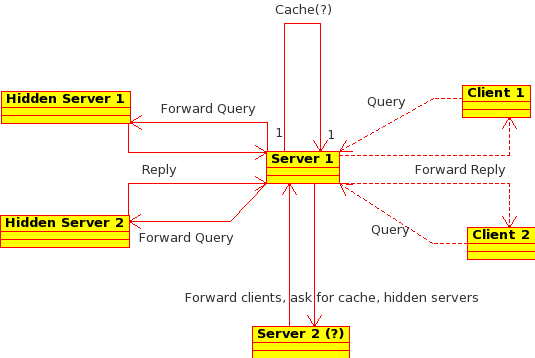
\includegraphics[width=\linewidth]{class_diagram}
\caption{Architektura}
\end{figure}
Komputer bez publicznego adresu IP (\emph{Hidden Server}) łączy się z serwerem
pośredniczącym (\emph{Server}). Gdy serwer pośredniczący dostaje od klienta (\emph{Client})
żądanie jakiegoś pliku, wysyła je do odpowiedniego Hidden Servera, który zwraca mu plik.
Następnie plik jest zwracany klientowi przez Server.
\subsubsection{Klienci/Serwery}
\begin{itemize}
\item Hidden Server --- komputer, który nie ma publicznego adresu IP, a chciałby hostować pliki.
Wbrew nazwie, jest on klientem, który łączy się z Serverem i udostępnia mu pliki.
\item Server --- komputer z publicznym adresem IP, który pośredniczy w wymianie plików między
Clientem a Hidden Serverem. Jest on niezbędny, gdyż jako jedyny posiada publiczny adres IP,
a co za tym idzie, można z nim nawiązać połączenie.
\item Client --- komputer, który jest zainteresowany dostępem do plików hostowanych przez
Hidden Server. Może, ale nie musi mieć publicznego adresu IP. Nawiązuje połączenie z Serverem.
\end{itemize}
\subsection{Możliwe dodatkowe funkcjonalności}
\subsubsection{Cache}
Server może przechowywać część często używanych plików w pamięci podręcznej. Gdy przychodzi
zapytanie o taki plik, wystarczy sprawdzić, czy wersja w cache jest najnowszą dostępną
wersją tego pliku (data modyfikacji).
\subsubsection{Wiele protokołów}
Server może obsługiwać wiele protokołów (HTTP, FTP\ldots). Warto zauważyć, że komunikacja 
między Serverem a Hidden Serverem jest w dużej mierze niezależna od protokołu jakim 
Client komunikuje się z Serverem (chociaż całe zapytanie Clienta mogło by być przekazywane 
do Hidden Servera w celu lepszej obsługi --- np. dostosowania pliku do języka Clienta).
\subsubsection{Wiele Serverów}
W celu zapewnienia lepszej skalowalności, można dodać więcej niż jeden Server. Wymaga
to opracowania dodatkowego protokołu, za pomocą którego Servery komunikowałyby się 
między sobą oraz rozwiązania problemu przekazywania obsługi zapytań klientów do mniej 
obciążonych Serverów.
\subsection{Protokoły}
Wszystkie protokoły mogą mieć polecenia przesyłane plain-textem, dla ułatwienia
implementacji i debugowania.
\subsubsection{Client --- Server}
Powinien to być jeden z publicznie znanych protokołów, aby Client nie musiał instalować
żadnego nowego oprogramowania). Najlepszym wyborem wydaje się być HTTP. 
Jak zostało wyżej wspomniane, nic nie stoi na przeszkodzie,
aby zaimplementować więcej niż jeden protokół.

\noindent Cechy tego protokołu są opisane w jego specyfikacji.
\subsubsection{Hidden Server --- Server}
Protokół powinien umożliwiać:
\begin{itemize}
\item żądanie jakiegoś pliku (Server wysyła żądanie, Hidden Server na nie odpowiada)
\item sprawdzenie daty ostatniej modyfikacji pliku (opcjonalnie --- przy dodaniu funkcjonalności cache)
\item żądanie cachowania jakiegoś pliku (opcjonalnie --- przy dodaniu funkcjonalności cache)
\item żądanie, żeby klient podłączył się do innego Servera (opcjonalnie --- przy dodaniu wielu Serverów)
\end{itemize}
Połączenie powinno być nawiązywane przez Hidden Server i utrzymywane tak długo, jak to jest
możliwe (po przerwaniu połączenia pliki hostowane przez Hidden Server znikają z sieci).

\noindent Cechy:
\begin{itemize}
\item zorientowany na połączenie (pliki hostowane przez Hidden Server są dostępne tylko
wtedy, gdy trwa połączenie).
\item bezstanowy --- ze względu na łatwość implementacji (żadne z wymagań nie 
wymusza użycia protokołu stanowego).
\item stworzenie osobnego kanału na dane zwiększyłoby wydajność i możliwości protokołu,
ale nie jest konieczne.
\end{itemize}
\subsubsection{Server --- Server (opcjonalnie --- przy wielu Serverach)}
Protokół powinien umożliwiać:
\begin{itemize}
\item przekazanie obsługi danego Hidden Servera do innego Servera
\item znalezienie Servera obsługującego dany Hidden Server (w celu przekierowania tam Clienta)
\end{itemize}
Połączenie powinno być zrywane po wykonaniu zadania.

\noindent Cechy:
\begin{itemize}
\item bezpołączeniowy (bo komunikacja między Serverami polega na wykonaniu pojedynczego zapytania)
\item bezstanowy (zapamiętywanie stanu nie jest potrzebne)
\item wspólny kanał na dane i polecenia (ilość przesyłanych informacji jest niewielka)
\end{itemize}

\subsection{Problemy}
Przy implementowaniu projektu trzeba będzie rozwiązać następujące problemy (a także 
wiele innych, których nie da się przewidzieć w tym momencie).
\begin{itemize}
\item Idealnie by było, żeby pobieranie pliku przez Clienta rozpoczęło się 
zanim plik zostanie w całości pobrany przez Server z Hidden Servera.
\item Istotny jest dobry wybór algorytmu cache'owania (opcjonalnie --- przy dodaniu funkcjonalności cache)
\item Ważny jest algorytm balansowania obciążenia Serverów (opcjonalnie --- przy wielu Serverach)
\item Problemem może być znajdowanie Servera, do którego aktualnie podłączony jest dany Hidden Server (opcjonalnie --- przy wielu Serverach)
\item Dokładne opracowanie protokołu Server --- Server (opcjonalnie --- przy wielu Serverach)
\end{itemize}

\end{document}
